\chapter{Introduction}\label{chap:introduction}

\epigraph{\emph{A program that is used and that, as an implementation of its specification, reflects some other reality, undergoes continuos change or becomes progressively less useful.
The change or decay process continues until it is judged more cost effective to replace the program with a recreated version.}}{--- Meir Lehman}

%\section{The relentless endeavor of software craftmanship}
\lettrine{T}{he} opening quote of this chapter is the first of the five laws of software evolution formulated by Lehman in the late 1970's \cite{Lehman1979}.
The law refers to the fact that all software is designed to operate in a specific enviroment and to satisfy a specific set of requirements. 
However, every enviroment, and every requirement, is bound to change eventually, rendering the software obsolete. %, unless it changes accordingly.
Therefore, the need of constantly adapting a software to new requirements, and shifts in the environment, is a \emph{relentless endeavor} that, over time, destabilises the sustainability of a software project.

A software project is \emph{sustainable} if the project owner is capable of applying whatever valuable change they ought to make, timely \cite{Winters2020}.
However, decisions and implementation choices made early on in the project's lifetime inevitably affect the decisions we have to make in the present, often making them harder.
Over time, as the system grows old, our capability of adapting the software to new requirements and changes in the enviroment grows narrower, and making changes becomes more expensive.
Eventually, the system becomes \emph{unsustainable} and the second part of Lehman's first law of software evolution comes into play.
In other words, a system that is unsustainable is a system that is \emph{poorly maintenainable} and with \emph{limited capabilities} to evolve. 

In 1992, Ward Cunningham cleverly adapted and reframed these concepts under term \emph{technical debt} \cite{Cunningham1992}. %TODO: improve this sentence
Since then, technical debt has gained a lot of traction among both practitioners and researchers alike.
Indeed, the presence of technical debt within a system is a problem that every non-trivial software system suffers from, and over the years, several studies have made great progress in identifying the causes and effects of technical debt \cite{Brown2010,Kruchten2012,Lehman1979}.
These materialised into the various forms, ranging from source code violations \cite{Letouzey2012,Curtis2012} and design level flaws \cite{Marinescu2012} to high-level decisions made at the architectural level \cite{Ernst2015,Yli-Huumo2014}.
In this regard, architectural smells (AS), defined as a \emph{``commonly (although not always intentionally) used architectural decisions that negatively impact system quality} \cite{Garcia2009} have gained a lot of attention from researchers over the past years \cite{Verdecchia2018}.
Although existing literature has devoted a considerable amount of effort to study AS \cite{Mo2015,Le2016,Arcelli2016}, our understanding of AS is still incomplete.

This dissertation aims at improving the current state of the art concerning our understanding of AS by answering questions such as: \emph{how are AS introduced?; how do AS evolve?; and, what is their impact on software maintenance (i.e. technical debt)?}

The fundamental proposition of this thesis is that a better understanding of AS will allow software practitioners to better manage technical debt.

In the upcoming sections, I will introduce the concepts of technical debt and architectural smells in further detail, as these are the \emph{leitmotif} of this dissertation.
I will also decompose the research problem addressed in this thesis into multiple research questions and the methodology used to answer them.


\section{Technical Debt}
In 1992, Cunningham first introduced the concept of \emph{technical debt} (TD) \cite{Cunningham1992}. 
The term was first coined to indicate the necessity of releasing software that, while it works perfectly, it does not meet the criteria of long-term sustainable software. 
Cunningham himself calls this an \emph{``unmasterable program''} that is \emph{``dangerous''} unless the \emph{debt} is repaid.
Unfortunately, TD repayment is not always feasible, as software practitioners have to work with limited time and budget, resulting in most of TD not being repaid \cite{Digkas2018}.
The time spent on not-quite-right code counts as \emph{interest} on that debt \cite{Cunningham1992}, making software projects more expensive to maintain.
Technical debt is a powerful metaphor that, essentially, conveys the importance of sustainable software -- and of Lehman's first law of software evolution -- in terms that are easy to understand and communicate to others. 
%Essentially, saying that a system has incurred a lot of technical debt, or that it is unsustainable, is saying that the system is \emph{poorly maintenainable} and with \emph{limited capabilities} to evolve. 

A modern definition of TD is the following: \emph{TD reflects the technical compromises that software practitioners make in order to achieve a short-term advantage at the expense of creating a technical context that increases complexity and cost in the long-term} \cite{Avgeriou2016}. 
Hence, a company can get into debt and, as long as it is aware of the debt and is planning to repay it in the medium-term period, leverage on it to temporarily increase productivity.
However, if the company is not aware that it is accruing TD, or does not repay it on time, the amount of interest may become too high, causing the failure of the project due to the huge cost of implementing changes.

During the course of the years, the metaphor has been extended by the research community and has assumed a wider meaning, englobing several aspects of the software development process like architecture, design, requirements, testing and documentation \cite{Brown2010}.
It is very hard to state a single definition that incorporates all the facets of such a big metaphor. 
But the current literature has explored the concept in all of its vastness and has proposed and analyzed multiple taxonomies and types of TD.
A common way of categorising TD is by the type of artefacts it affects. Using this approach, Li et al. identified several different types of TD \cite{Li2015}, namely \emph{Requirements TD}, \emph{Architectural TD}, \emph{Design TD}, \emph{Code TD}, \emph{Test TD}, \emph{Build TD}, \emph{Documentation TD}, \emph{Infrastructure TD}, and \emph{Versioning TD}.

% TODO: finish this section


\section{Architectural smells}

% \subsection{Why smells over existing metric?}

\section{The project SDK4ED}

\section{Research design}
\subsection{Problem statement}
In the early years of the research on architectural smells, researchers focused on identifying new types of smells, theoretical define each smell, propose a detection rule, and finally describe their impact on software maintenance from a theoretical point of view \cite{Lippert2006,Garcia2009,Mo2015,Le2016,Arcelli2016}.
From there, researchers moved on to study how smells impact software maintenance in open source systems \cite{Choudhary2016,Xiao2016,Le2018}, study their interaction with other types of smells \cite{Sharma2017,Arcelli2019}, and even predict their introduction in future releases \cite{Arcelli2019b}.
All of these studies offer a great insight into the theoretical nature of architectural smells, and some of them even provide limited evidence to support whether the hypothesized negative effects on software maintenance are detectable in real world systems.
However, there are still three important research threads that are either incomplete or not investigated at all:
\begin{enumerate}
    \item there are no specific details on how individual architectural smell instances evolve over time. This means that it is not clear how architectural smells are \emph{introduced}, how long they \emph{persist} within the system, and whether any TD interest is \emph{paid} on the components affected by architectural smells; 
    \item no studies investigate how architectural smells are \emph{perceived} by practitioners. This means that thare is little to no empirical evidence on how architectural smells concretely affect the work of software developers and architects;
    \item only a few studies investigate the possibility to \emph{estimate} the amount of technical debt principal generated by architectural smells. But these approaches either lack an industrial validation or use limited approaches to estimate it. 
\end{enumerate}
If architectural smells are to be used by practitioners to manage TD, these three research areas are of paramount importance in order to achieve that.
%The lack of research in these three areas severly limits the application of architectural smells in practice.

The three points highlighted above can be summarised under the following problem statement:
\begin{quote}
    ``Existing literature on architectural smells does not document how AS are introduced, how long they persist, and how software practitioners are impacted by AS. 
    This limits existing implementations of a fully-automated, data-driven approach to manage the technical debt generated by architectural smells.''
\end{quote}

\subsection{Design science and research methodology}

\subsection{Problem decomposition}
\begin{figure}
    \centering
    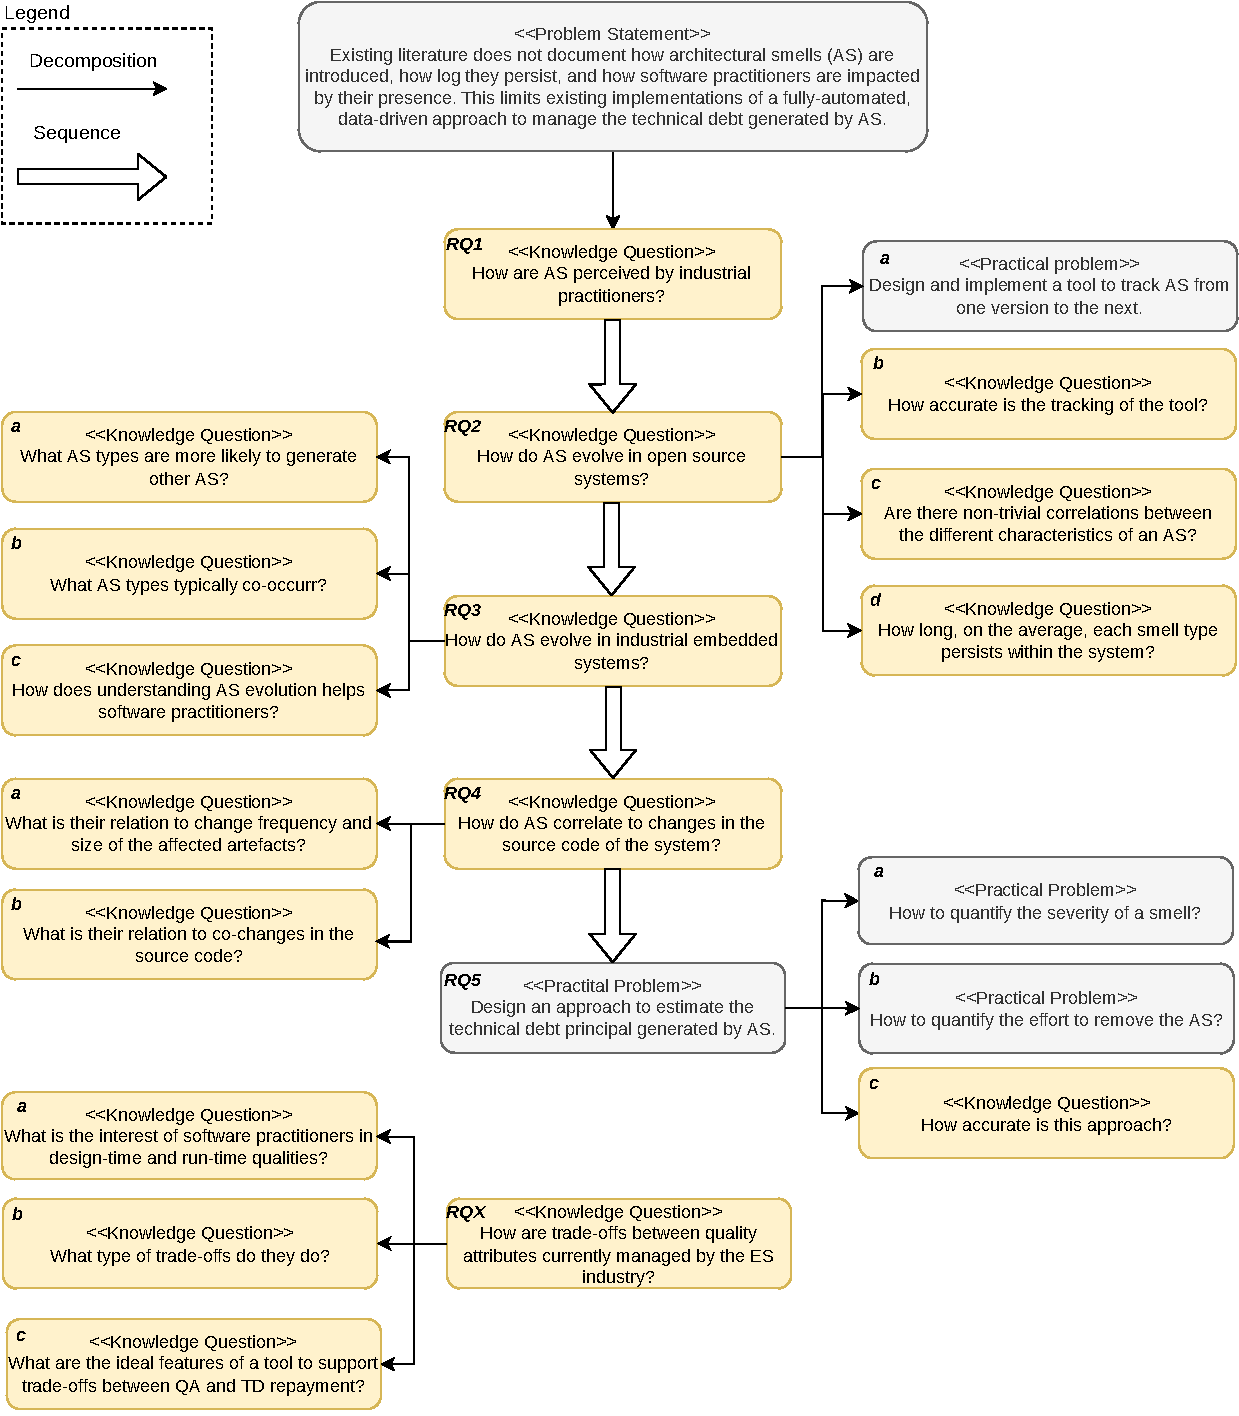
\includegraphics[width=\textwidth]{c1/design-science.pdf}
    \caption{A caption}\label{fig:problem-decomposition}
\end{figure}
\subsection{Overview of this dissertation}

